\section{Auswertung}
\label{sec:Auswertung}

\subsection{Energiekalibrierung}

Zur Energiekalibrierung des Detektors wird das Spektrum eines $\ce{^{152}Eu}$-Strahlers aufgenommen, welches in Abbildung
\ref{fig:plot1} zu sehen ist.

\begin{figure}
  \centering
  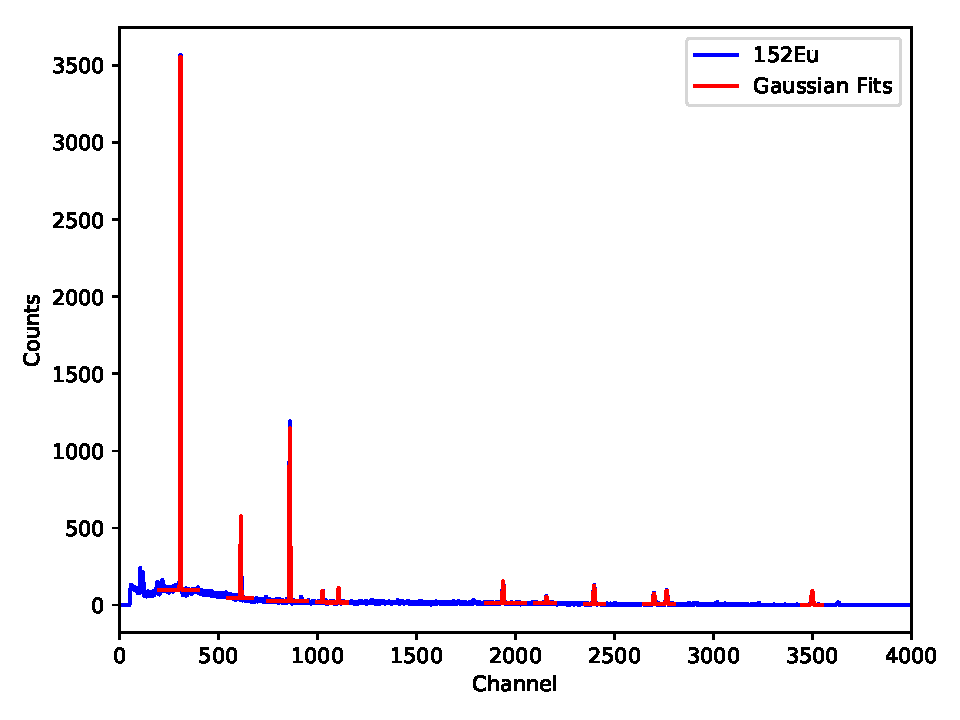
\includegraphics{content/plot1.pdf}
  \caption{Gemessenes Spektrum eines $\ce{^{152}Eu}$-Strahlers}
  \label{fig:plot1}
\end{figure}

Dazu werden anhand der charakteristischen Peaks des Spektrums mittels linearer Regression Peakenergien $E_i$ und mittlere 
Kanalnummern $\mu_i$ in Beziehung gesetzt.
Die Peaks werden als Gaußverteilungen der Form 

\begin{equation}
  f(x) = a \cdot \text{exp}\left( - \frac{(x-\mu_i)^2}{b}\right) + c
\end{equation}

genähert. Dazu wird die Funktion \textit{scipy.optimize.curve\_fit} aus der Python-Bibliothek SkiPy verwendet.

Die den Peakenergien $E_i$ zugeordneten Näherungsparameter sind in Tabelle \ref{tab:mess1} aufgelistet.

\begin{table}
  \centering
  \caption{Gefittete Parameter der Gaußnäherungen der charakteristischen Peaks des $\ce{^{152}Eu}$-Spektrums}
  \label{tab:mess1}
  \sisetup{table-format=2.1}
  \begin{tabular}{c c c c c}
  \toprule
  $ E_i \;/\; \si{\kilo\eV}$ & $\mu_i$ & $a$ & $b$ & $c$ \\
  \midrule
        121,78 &  308,80 $\pm$ 0,01 & 3493,0 $\pm$ 15,0 &  3,5 $\pm$ 0,0 & 100,3 $\pm$ 1,3 \\
        244,70 &  613,80 $\pm$ 0,03 &  535,0 $\pm$  9,0 &  4,2 $\pm$ 0,2 &  45,6 $\pm$ 1,1 \\
        344,30 &  860,70 $\pm$ 0,01 & 1140,0 $\pm$  6,0 &  5,5 $\pm$ 0,1 &  24,4 $\pm$ 0,6 \\
        411,12 & 1026,51 $\pm$ 0,09 &   74,7 $\pm$  3,5 &  5,7 $\pm$ 0,6 &  18,9 $\pm$ 0,8 \\
        443,96 & 1107,93 $\pm$ 0,06 &   94,2 $\pm$  3,0 &  6,4 $\pm$ 0,5 &  16,7 $\pm$ 0,5 \\
        778,90 & 1938,62 $\pm$ 0,05 &  143,3 $\pm$  2,4 & 14,3 $\pm$ 0,5 &  11,7 $\pm$ 0,3 \\
        867,37 & 2158,39 $\pm$ 0,17 &   42,5 $\pm$  2,1 & 17,1 $\pm$ 2,0 &  10,7 $\pm$ 0,4 \\
        964,08 & 2398,18 $\pm$ 0,06 &  120,3 $\pm$  2,2 & 19,3 $\pm$ 0,8 &   6,4 $\pm$ 0,5 \\
       1085,90 & 2700,41 $\pm$ 0,14 &   67,5 $\pm$  2,2 & 30,2 $\pm$ 2,3 &   5,3 $\pm$ 0,5 \\
       1112,10 & 2765,02 $\pm$ 0,11 &   88,5 $\pm$  2,6 & 23,2 $\pm$ 1,7 &   5,6 $\pm$ 0,9 \\
       1408,00 & 3499,69 $\pm$ 0,07 &   90,7 $\pm$  1,4 & 28,9 $\pm$ 1,1 &   0,9 $\pm$ 0,3 \\
  \bottomrule
  \end{tabular}
  \end{table}

Mit den Wertepaaren der Peakenergien $E_i$ und der mittleren Kanalnummern $\mu_i$ wird eine lineare Regression der Form

\begin{equation}
  E_i(\mu_i) = m \cdot \mu_i + d
\end{equation}
  
durchgeführt, die in Abildung \ref{fig:plot5} dargestellt ist.
Die Regressionsparameter betragen

\begin{align*}
  m &= 0.403 \pm 0.000 \\
  d &= -2.683 \pm 0.051
\end{align*} \; .

\begin{figure}
  \centering
  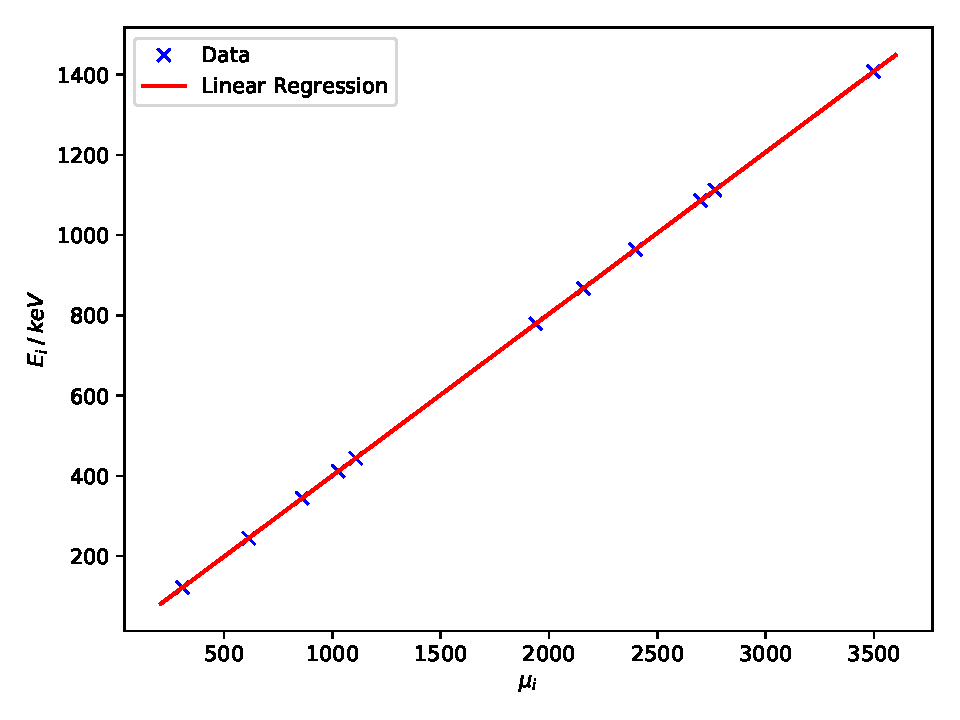
\includegraphics{content/plot5.pdf}
  \caption{Lineare Regression der Energie-Kanalnummer-Wertepaare des $\ce{^{152}Eu}$}
  \label{fig:plot5}
\end{figure}
